\documentclass[10pt,dvipsnames]{beamer}
\usepackage{amsmath,amssymb,longtable,hhline}
\usepackage{mathrsfs}
\usepackage{xcolor}
\usepackage{hyperref}
\usepackage{multicol}
\usepackage{anyfontsize}
\usepackage{minted}

\usemintedstyle{tango}
\newcommand{\ltprgsize}{\fontsize{5}{5}\selectfont}
\setminted{fontsize=\ltprgsize,mathescape}

\definecolor{mygreen}{rgb}{0,0.6,0}
\definecolor{mygray}{rgb}{0.5,0.5,0.5}
\definecolor{mymauve}{rgb}{0.58,0,0.82}

\hypersetup{
    bookmarks=true,         % show bookmarks bar?
    unicode=true,           % non-Latin characters in Acrobat’s bookmarks
    pdftoolbar=false,        % show Acrobat’s toolbar?
    pdfmenubar=false,        % show Acrobat’s menu?
    pdffitwindow=false,     % window fit to page when opened
    pdfstartview={FitH},    % fits the width of the page to the window
    pdftitle={Компьютерная алгебра в задачах оптимизации},    % title
    pdfauthor={Evgeny Cherkashin, Seseg Badmatsyrenova},     % author
    pdfsubject={symbolic computations},   % subject of the document
    pdfnewwindow=true,      % links in new PDF window
    colorlinks=true,       % false: boxed links; true: colored links
    linkcolor=red,          % color of internal links (change box color with linkbordercolor)
    citecolor=green,        % color of links to bibliography
    filecolor=magenta,      % color of file links
    urlcolor=blue           % color of external links
}

\usepackage{pifont}

\usetheme{Warsaw}
\usecolortheme{crane}
%\useinnertheme{rectangles}
\setbeamertemplate{itemize item}{\scriptsize\hbox{\donotcoloroutermaths\ding{113}}}
\setbeamertemplate{itemize subitem}{\tiny\raise1.5pt\hbox{\donotcoloroutermaths$\blacktriangleright$}}
\setbeamertemplate{itemize subsubitem}{\tiny\raise1.5pt\hbox{\donotcoloroutermaths$\blacktriangleright$}}
\setbeamertemplate{enumerate item}{\insertenumlabel.}
\setbeamertemplate{enumerate subitem}{\insertenumlabel.\insertsubenumlabel}
\setbeamertemplate{enumerate subsubitem}{\insertenumlabel.\insertsubenumlabel.\insertsubsubenumlabel}
\setbeamertemplate{enumerate mini template}{\insertenumlabel}

\beamertemplatenavigationsymbolsempty

\usepackage{iftex,ifxetex}
\ifPDFTeX
  \usepackage[utf8]{inputenc}
  \usepackage[T1]{fontenc}
  \usepackage[russian]{babel}
  \usepackage{lmodern}
  \usefonttheme{serif}
\else
  \ifluatex
    \usepackage{unicode-math}
    \defaultfontfeatures{Ligatures=TeX,Numbers=OldStyle}
    \setmathfont{Latin Modern Math}
    \setsansfont{Linux Biolinum O}
    \setmonofont{Fira Mono}
    \usefonttheme{professionalfonts}
    % \setmathfont[
    %     Ligatures=TeX,
    %     Scale=MatchLowercase,
    %     math-style=upright,
    %     vargreek-shape=unicode
    %     ]{euler.otf}
  \fi
\fi

%\useoutertheme{split}
%\useinnertheme{rounded}
\setbeamertemplate{background canvas}[vertical shading][bottom=white!80!cyan!20,top=cyan!10]
%\setbeamertemplate{sidebar canvas left}[horizontal shading][left=white!40!black,right=black]

\graphicspath{{pics/}}


% --------------------------

\def\remph#1{\textcolor{Mahogany}{\bfseries #1}}
\newcommand{\irnitu}{INRTU}
\newcommand{\inrtu}{INRTU}

\begin{document}
\parindent=1em
\title{Recommender systems for career guidance}
\author{
\def\and{, }
Trần Đức Thế\and
\remph{Evgeny~Cherkashin}\and
Viktoria Kopylova\and
Nikita Lukyanov}


\date{${}$\\\vspace{2em}AIIT-2021, October, 15}
\institute{\textit{Matrosov Institute for System Dynamics and Control Theory of SB RAS}, Irkutsk, Russia,
  \href{mailto:eugeneai@icc.ru}{eugeneai@icc.ru}\\
  \textit{National research Irkutsk state technical university (\irnitu),} Irkutsk, Russia,\\
  \href{mailto:kopylovika@mail.ru}{kopylovika@mail.ru}}

\maketitle
% ----------------------------------------------------------------
\begin{frame}{Introduction}

  \emph{Recommender systems} (RS) are \emph{decision support systems}. They are useful to support users with additional information and decision variants.  We consider two RS in career guidance field.

Both systems were developed within master degrees at Institute for Information Technologies and Data Analysis, National research Irkutsk state technical university.

\textbf{Relevance} is justified by
\begin{itemize}
\item In the \textbf{countries with young population}, such as Việt Nam, the \textbf{demand of young specialists is high}. In fact, quite often graduates remain unemployed for a long time or do not work in originally mastered specialties.
\item \textbf{University} institutions \textbf{are interested in rising quality of entrants}: attract attention of domain targeted students with high potentials to the existing courses, organize new courses for target student groups.
\end{itemize}

%In the \textbf{second} RS entrants are to obtain perspective specialty, comfort to their nature.  There are no industry supporting career guidance, only informational services and neighbors' subjective experience.  The universities' activities should be focused to a target audience with supplying students \textbf{relevant optional courses}.


\end{frame}

\begin{frame}
  \frametitle{Interest assessment}
  In the tables, we present the result of interest assessment to career guidance and relevance of improving of the guidance system.
\begin{table}[thb]
  \caption{Interest assessment to the carer guidance in Việt Nam, Hà Tĩnh city}
  \label{tab:interest}
  \centering
  \begin{tabular}{|l|c|c|}
    \hline
    \textbf{Interest level} & \textbf{Count of votes} & \textbf{Ratio, \%} \\
    \hline
    Very interested & 218 & 51.9 \\
    \hline
    Relatively interested & 155 & 36.9 \\
    \hline
    Less interested & 36 & 8.6 \\
    \hline
    No interest & 11 & 2.6 \\
    \textbf{Total} & \textbf{420} & \textbf{100} \\
    \hline
  \end{tabular}
\end{table}

\begin{table}[bht]
  \caption{Questionary results of middle school students on need for improvement of the carer guidance system}
  \label{tab:interest}
  \centering
  \begin{tabular}{|l|c|c|}
    \hline
    \textbf{Answer option} & \textbf{Quantity} & \textbf{Ratio, \%} \\
    \hline
    very necessary & 272 & 64.8 \\
    \hline
    necessary & 145 & 34.5 \\
    \hline
    no necessity & 3 & 0.7 \\
    \hline
    \textbf{Total} & \textbf{420} & \textbf{100} \\
    \hline
  \end{tabular}
\end{table}
\end{frame}

\begin{frame}
  \frametitle{Background}
  \begin{columns}
    \begin{column}{0.5\linewidth}
      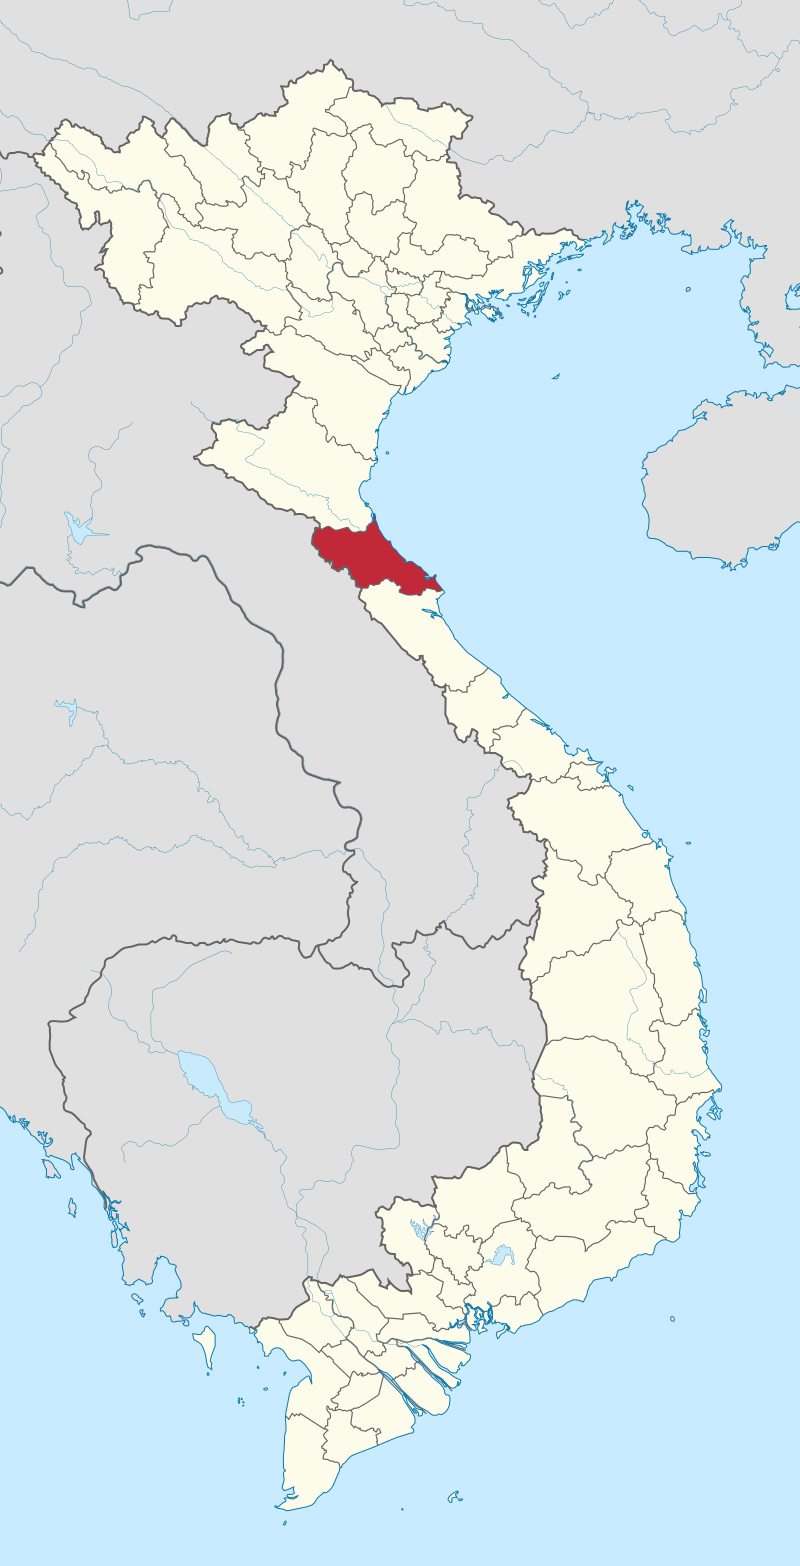
\includegraphics[width=0.75\linewidth]{pics/Ha-Tinh.png}
    \end{column}
    \begin{column}{0.5\linewidth}
      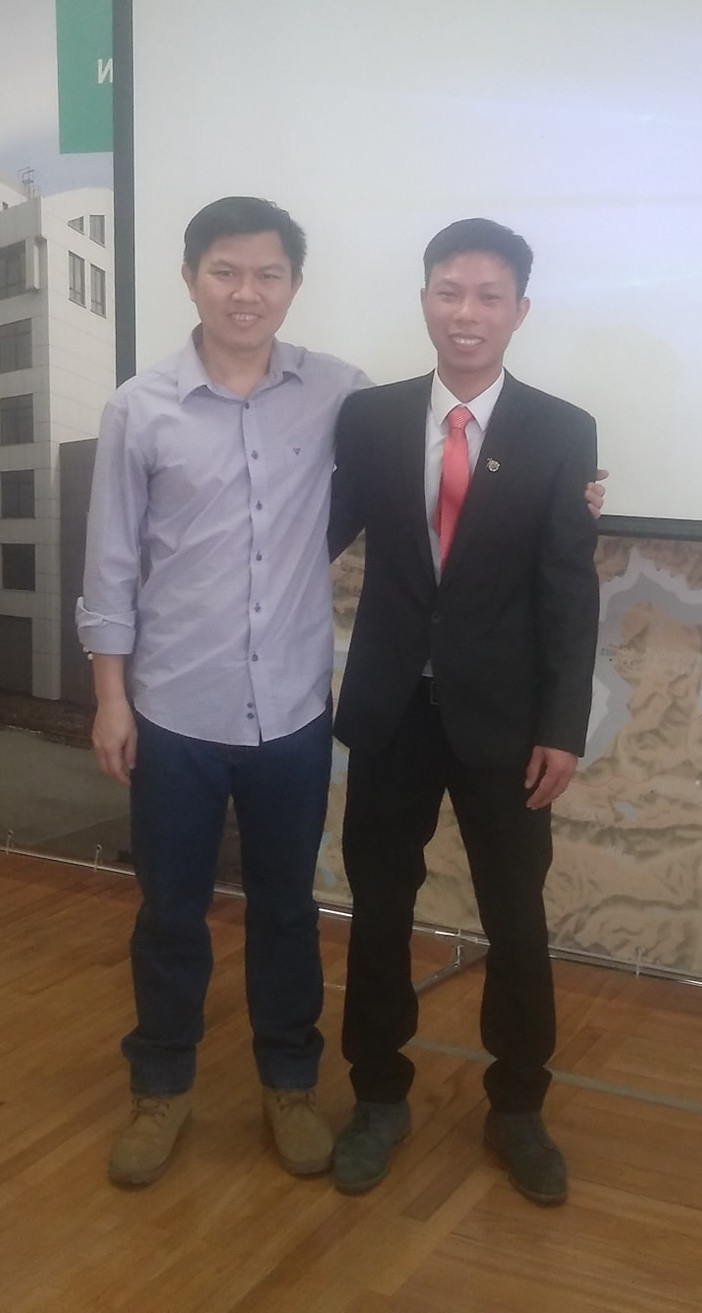
\includegraphics[width=0.8\linewidth]{pics/the-and-student.jpg}
    \end{column}
  \end{columns}
\end{frame}

\begin{frame}
  \frametitle{RS classification by solved problems}
  \begin{enumerate}
  \item \textbf{Increasing} the \textbf{sales} of a product
    \begin{itemize}
    \item a \textbf{number} of commodities sold
    \item organizing \textbf{wider range} product sales
    \end{itemize}
  \item \textbf{Increasing} user \textbf{satisfaction} and/or loyalty
  \item Better understanding \textbf{user needs}
  \item \textbf{Better products offers} with respect to the user needs
  \item Selection of sets of \textbf{products} for users \textbf{with common properties}
    \begin{itemize}
    \item ``good'' ones, and
    \item product groups, having a common usability properties
    \end{itemize}
  \item Mining the classes of products, \textbf{structuring} the RS \textbf{product domain}, and
  \item Generate a \textbf{continuity of recommendations} using the classification
  \item \textbf{Rectifying user profile}, \emph{e.g.} with targeted questioning
  \item For the users having no goal to make a choice, but searching for expert opinions
    \begin{itemize}
    \item \textbf{Analysis of} other \textbf{users impact} on a choice
    \item Formalizing opinions
    \item Recommending opinions
    \end{itemize}
  \end{enumerate}
\end{frame}

\begin{frame}
  \frametitle{General stages of RS design and implementation}
  RS development is being carried on according to the following scenario:
  \begin{enumerate}
  \item Investigation of the domain and defining the \textbf{users} and \textbf{objects} of recommendation.
  \item Determine the \textbf{sources} of information.
  \item Develop techniques for solving ``\textbf{cold start}'' problems.
  \item Propose \textbf{methods and algorithms of comparing} objects and users, and their \textbf{mutual relations}.
  \item Implement data structures, storage, analysis and synthesis algorithms.
  \item Testing.
  \end{enumerate}
  In both systems \textbf{users} are \textbf{middle school students}, \textbf{entrants}, and \textbf{high school students}.  \textbf{Objects} are references to professions expressed as \textbf{universities and their departments}.
\end{frame}

\begin{frame}
  \frametitle{Sources of information: \emph{collecting refinement data}}
  \begin{columns}
    \begin{column}{0.4\linewidth}
      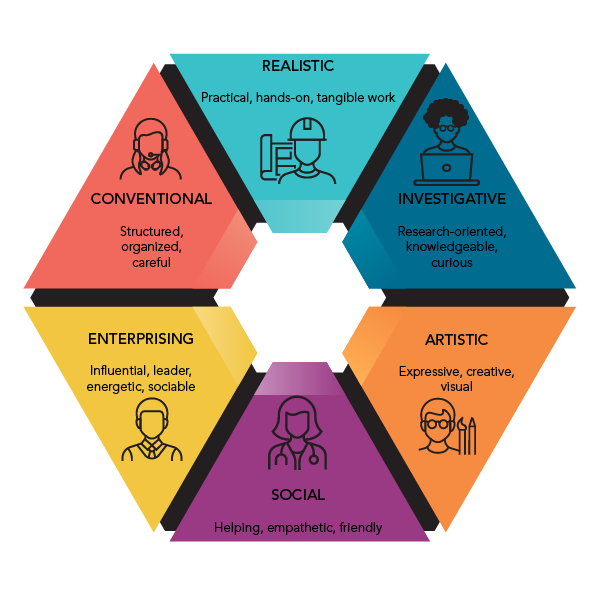
\includegraphics[width=0.9\linewidth]{pics/holland_hexagon.png}
      {\tiny\url{https://letstalkscience.ca/educational-resources/lessons/work-interests-and-holland-code}}
    \end{column}
    \begin{column}{0.6\linewidth}
      \begin{enumerate}
      \item Application of John Holland's Six Interest Types Technique for \textbf{structuring} school students' \textbf{interests}. This requires 54 questions to be answered.
      \item Relate local universities to the types by
      \item obtaining students' ratings on universities
      \end{enumerate}
      Then the resulting recommendations will be generated as Top-$N$ from an interest type.

      Thus, the \textbf{cold start} problem has been solved mostly by applying \textbf{expert knowledge}.
    \end{column}
  \end{columns}
\end{frame}

\begin{frame}
  \frametitle{Sources of information: \emph{social network data}}
  \textbf{Social networks} are popular ways of self-expression for school students and entrants.  User's properties are the profile data and set of group and channel subscriptions represented with \textbf{tags, keywords}.  TSU\footnote{Tomsk State University, Tomsk Russia} research showed that `In Contact'  (В Контакте) students profiles are closely related to educational interests.

  \begin{enumerate}
  \item Students of first three courses were asked their In Contact profile names. (\textbf{6270} from \textbf{7 institutes of \irnitu{}})
  \item The profile data were obtained via In Contact API (\textbf{4325, 68.98\%}, \textbf{480 features}).
  \item Data were filtered
    \begin{itemize}
    \item Removed inaccessible `private' profiles (\textbf{686})
    \item Removed content prohibited by law (\textbf{389} features)
    \end{itemize}
  \end{enumerate}

  Students' distribution among \irnitu{} institutes was obtained by means of \textbf{parsing enrollment documents}.  Enrollments will be related to the set of subscriptions and other profile characteristics (features).

  This solves \textbf{cold start} problem as well.

  % Recommendations are to be produced with machine learning. \emph{e.g.}, a neural network (NN), pretrained to relate user class to a specialty [class].  Another NN will be used to distribute new entrants to classes.
\end{frame}

\begin{frame}
  \frametitle{Object and user comparison}
  Pearson correlation was applied to the user ratings of universities and the correlation matrix were produced, $r_{u,j}$ is a rating of $u$-th user given for $i$-th university.
  $$sim(i,j)=\frac{\sum_{u\in U}(r_{u,i}-\bar{r}_i)(r_{u,j}-\bar{r}_j)}{\sqrt{\sum_{u\in U}(r_{u,i}-\bar{r}_i)^2}\sqrt{\sum_{u\in U}(r_{u,j}-\bar{r}_j)^2}}$$ % Page 18 The
  % Page 52 The

The correlation matrix for the universities is obtained similarly.

  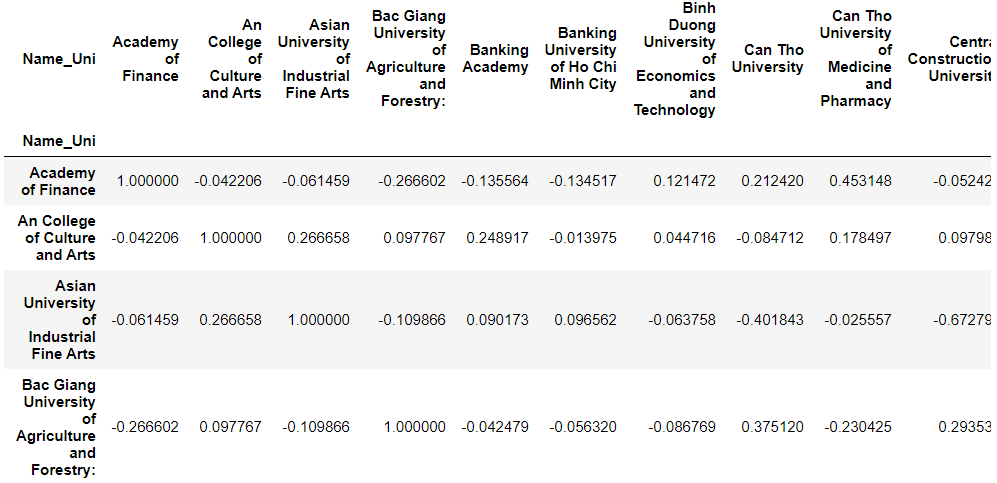
\includegraphics[width=\linewidth]{pics/ratings-corr.png}
\end{frame}

\begin{frame}
  \frametitle{Relating \irnitu{} institutes with students}
  Experiments were carried on to figure out the best feature set to be used in train set, namely,
  \begin{itemize}
  \item Induce a taxonomy of subscription group by application of a hierarchical clustering.
  \item Explore informative values of the groups as features by application of principal component analysis.
  \item Deduce the values with construction of a decision tree.
  \end{itemize}
  \vspace{2em}
  \centering
  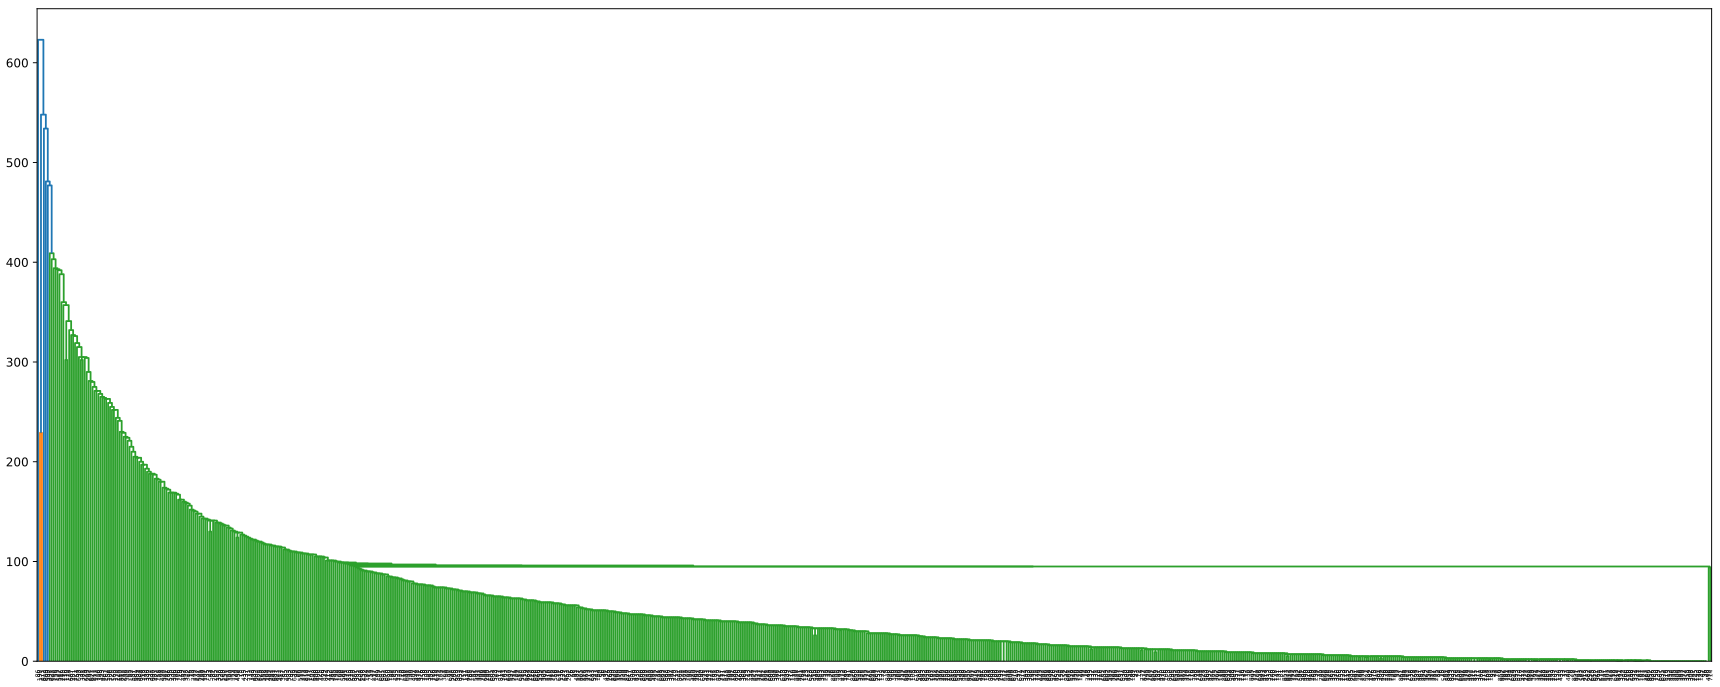
\includegraphics[width=0.8\linewidth]{pics/hclustering.png}
\end{frame}

\begin{frame}
  \frametitle{Principal Component Analysis}
  \begin{columns}
    \begin{column}{0.4\linewidth}
      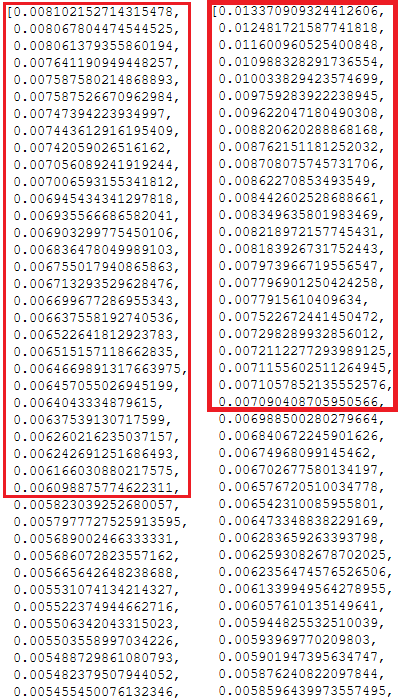
\includegraphics[width=\linewidth]{pics/pcas.png}
    \end{column}
    \begin{column}{0.6\linewidth}
      The chosen features by the red rectangles are the sets with the same informative `capabilities'.\\[1em]

      There are no explicit set of features, describing varieties of data for PC1 and PC3.
    \end{column}
  \end{columns}
\end{frame}

\begin{frame}
  \frametitle{Decision trees}
  \centering
  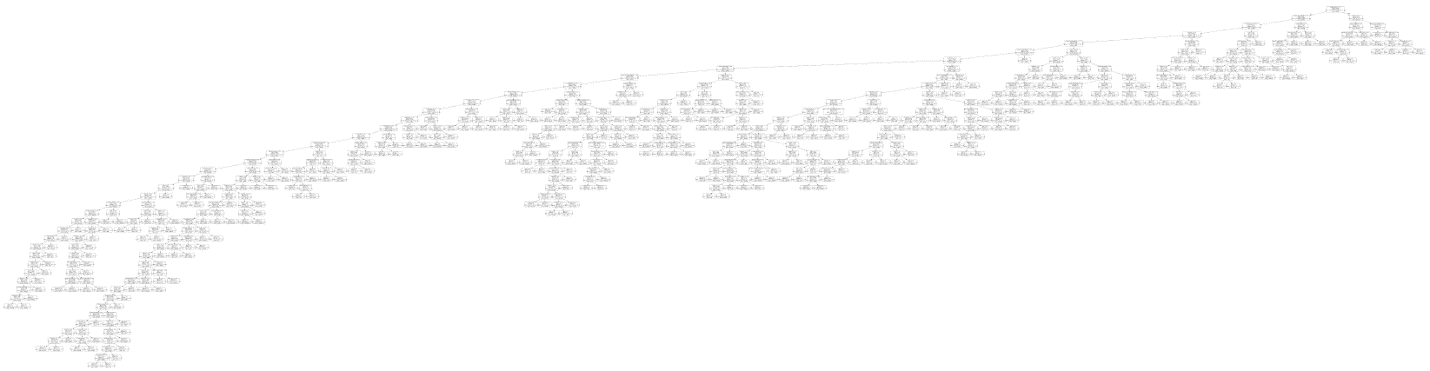
\includegraphics[width=\linewidth]{pics/long-tree.png}
  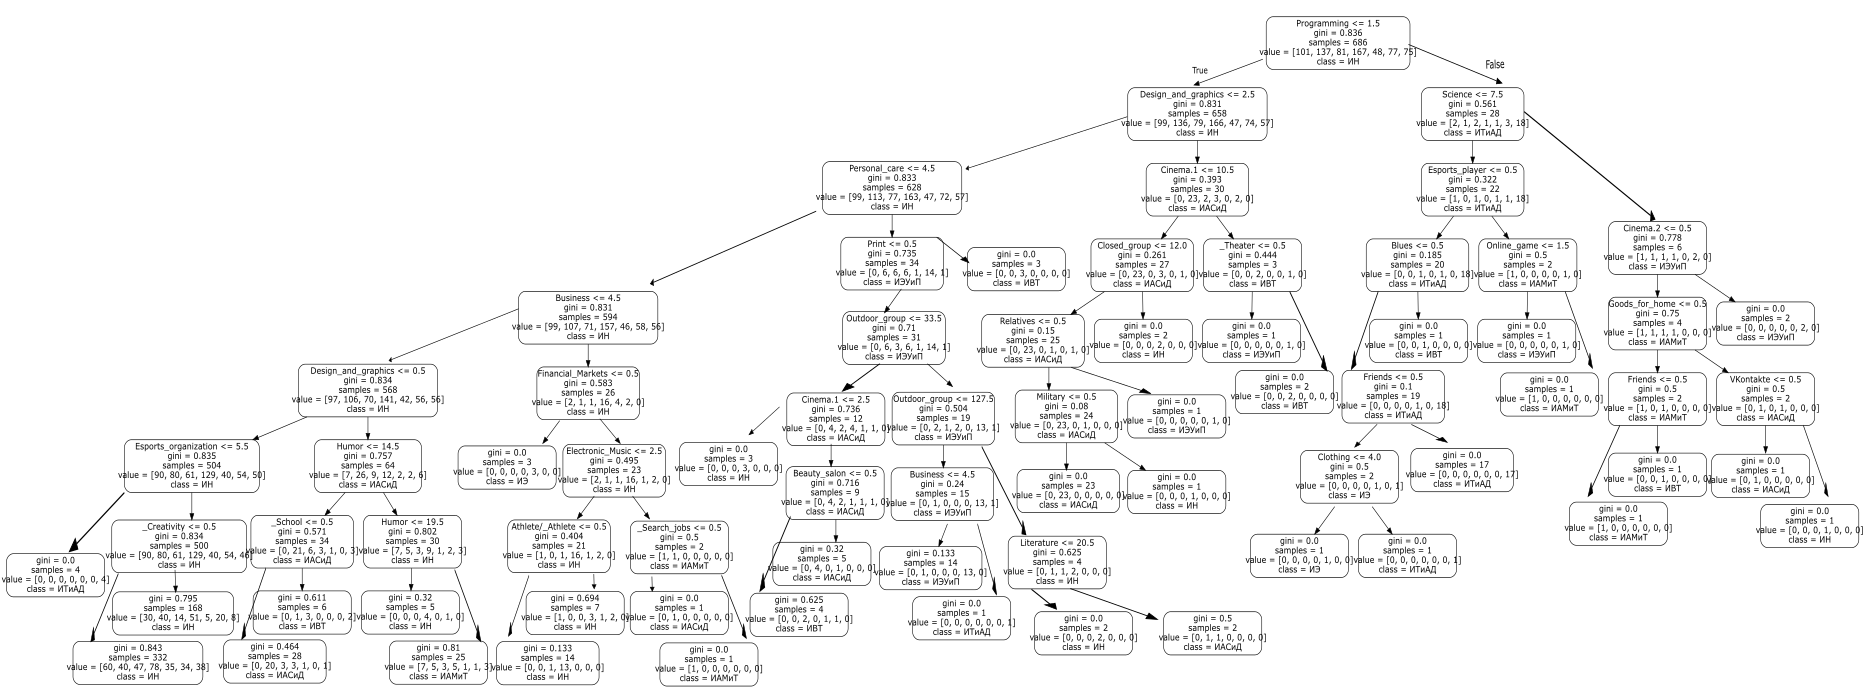
\includegraphics[width=\linewidth]{pics/7-level-tree.png}
\end{frame}

\begin{frame}
  \frametitle{Decision trees}
  The top-13 features describe only 20\% of phenomena.
  \begin{itemize}
  \item Programming
  \item Design \& graphics
  \item Personal care
  \item Cinema.1 (probably novel, documental)
  \item Science
  \item Sports player
  \item Print, Theater, Blues, Online games, Cinema.2 (probably fantastic)
  \end{itemize}
  \centering
  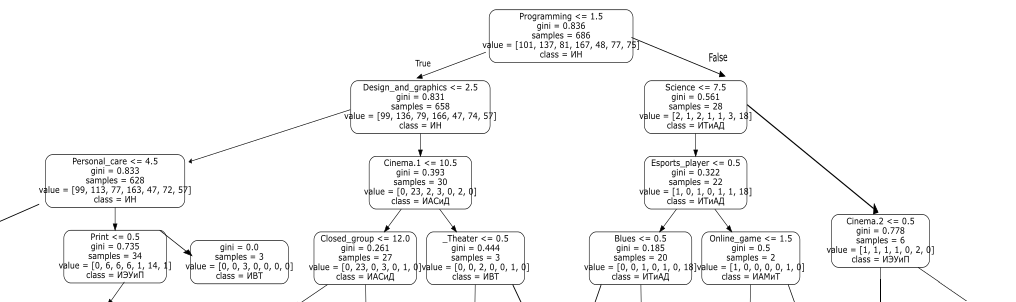
\includegraphics[width=\linewidth]{pics/top-features.png}
\end{frame}

\begin{frame}
  \frametitle{Artificial Neural Nets}
  \begin{columns}
    \begin{column}{0.3\linewidth}
      The training results\\[1em]
      \texttt{\tiny
        Best precision: 23.96\%\\
        Best model: FastForestOva\\
        Training time: 84\ 008 sec\\
        Models explored: 14\\[1em]
        Library: ML.NET
      }
    \end{column}
    \begin{column}{0.7\linewidth}
      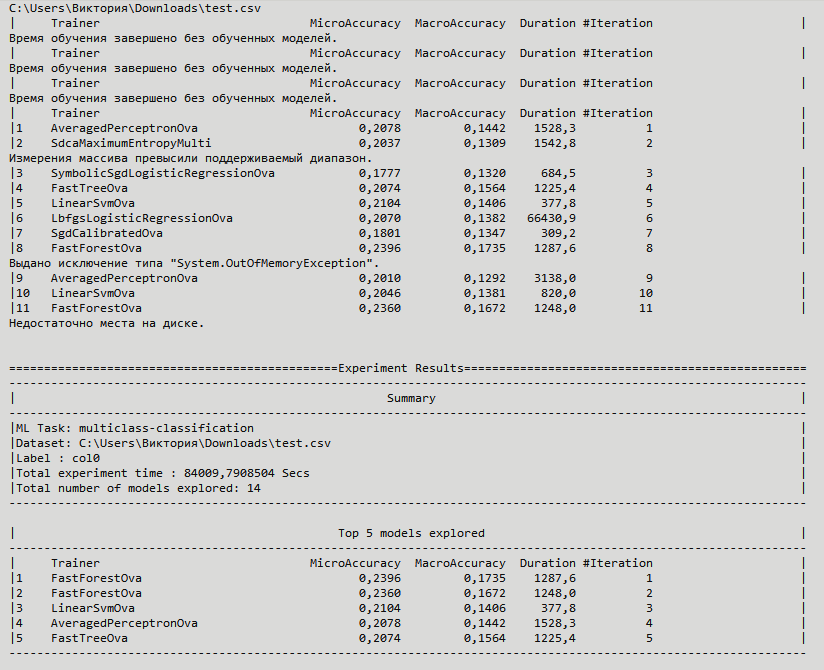
\includegraphics[width=\linewidth]{pics/nn-set.png}
    \end{column}
  \end{columns}
\end{frame}

\begin{frame}
  \frametitle{Resulting neural model}
  \begin{columns}
    \begin{column}{0.5\linewidth}
      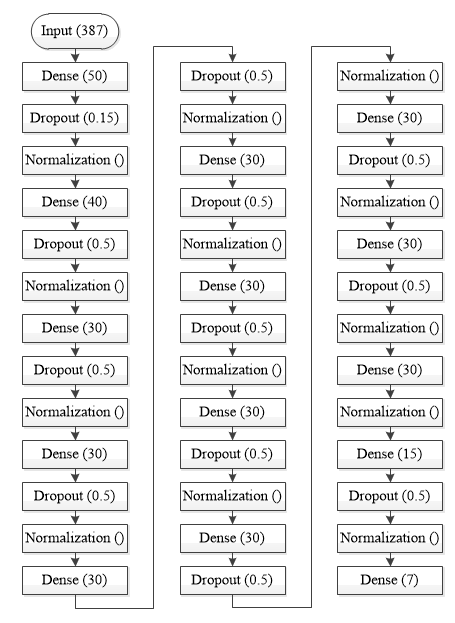
\includegraphics[width=\linewidth]{pics/algo.png}
    \end{column}
    \begin{column}{0.5\linewidth}
      \
      \begin{itemize}
      \item One multilayer neural network.
      \item Recommending \textbf{four} directions instead \textbf{one}
      \item Precision: 86\% (testing set) 22\% (learning set)
        \item Library: Keras (Python)
      \end{itemize}
      \vspace{2em}
      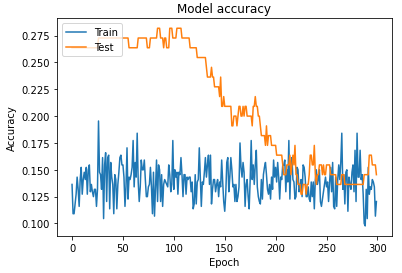
\includegraphics[width=\linewidth]{pics/accuracy.png}
    \end{column}
  \end{columns}

\end{frame}

\begin{frame}
  \frametitle{Testing}
  \centering
  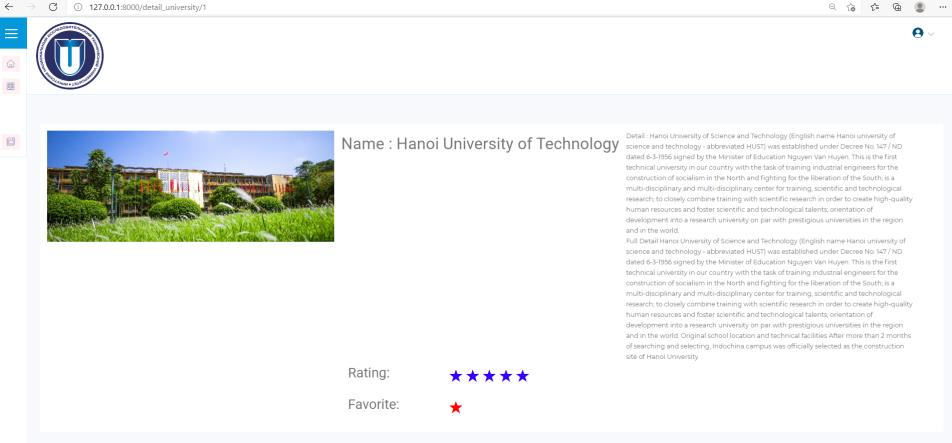
\includegraphics[width=0.7\linewidth]{pics/1-rating.png}
  \vspace{1em}
  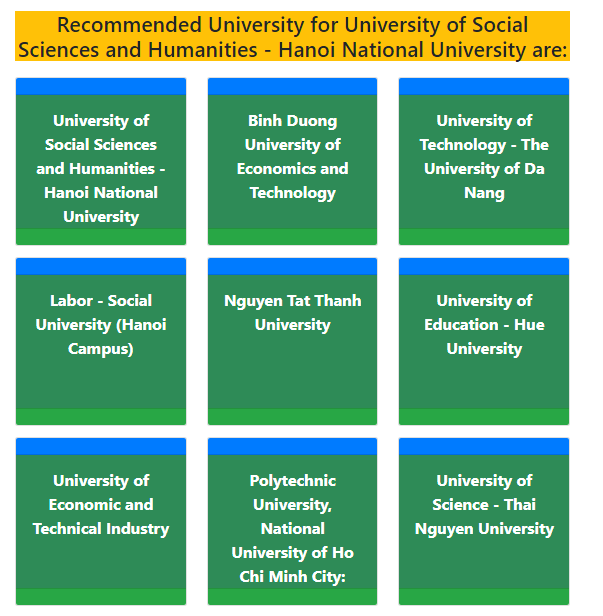
\includegraphics[width=0.5\linewidth]{pics/1-example.png}

\end{frame}

\begin{frame}
  \frametitle{Testing}
  \begin{columns}
    \begin{column}{0.5\linewidth}
      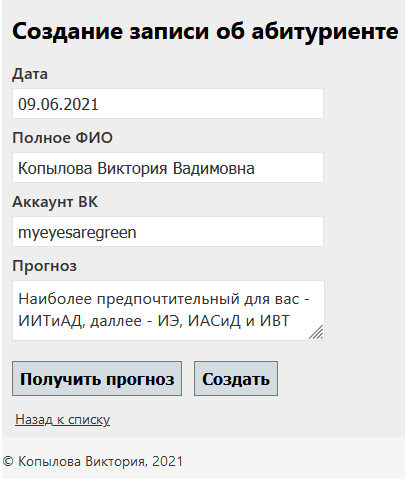
\includegraphics[width=\linewidth]{pics/2-example.png}
    \end{column}
    \begin{column}{0.5\linewidth}
      Stages of recommendation generation
      \begin{enumerate}
      \item Access In Contact account via API
      \item Load subscriptions and profile data
      \item Conversion to features
      \item Apply neural net for classification
      \item Print output
      \end{enumerate}
    \end{column}
  \end{columns}
\end{frame}

% \begin{frame}
%   \frametitle{Implementation}
%   \begin{itemize}
%   \item
%   \end{itemize}
% \end{frame}

\begin{frame}
  \frametitle{Discussion}

  Ha Tinh RS provides top-6 universities and was not measured on required criteria (precision, recall). It is intended to use as a web pages on the site of a Việt Nam school, and its purpose is in interpretation of the J.~Holland's technique.

  For the \irnitu{} RS some analysis of the results was carried out.
  \begin{itemize}
  \item The wrongly classified (out of 86\% precision) test set contained 9 students, which stopped studying, 3 study economics at IT institution, and for 7, no explanation were found.
  \item There are institutes having too wide set of specialties even contradictory to their generic intention. \emph{E.g.} \textbf{IIT\&DA} (our institute) have economics as a direction, \textbf{IAM\&T} does not limit itself with aircraft engineering, engineering general and computer graphics.
  \end{itemize}

The TGU's hypothesis on well correlated set of subscriptions and faculty direction was \textbf{not confirmed}, so a deep learning have to be used to obtain `good' model.

\end{frame}

\begin{frame}
  \frametitle{Conclusion}
  We presented results of two master degree projects.  Both are finished, and present somewhat different approaches to solve problems in a common domain of career guidance.
  \begin{enumerate}
  \item Authors carried out all necessary stages for producing techniques for RS software design.
  \item The proposed techniques were implemented, using popular web frameworks.
  \item Analysis of the results with different level of detail has been provided.
  \item Recommender system MVP-s were constructed for introduction into school career guidance.
  \end{enumerate}

\end{frame}


\begin{frame}{}
  \vfill
  \centering
  \Huge \textbf{Thank You for attention!}
  % \vfill
  % 
\includegraphics[width=0.5\linewidth]{QRURL.png}\\
  % \normalsize\url{https://github.com/eugeneai/papers-aiit-rs/raw/master/talk-2020-10-16-RS.pdf}
\end{frame}

\end{document}


%%% Local Variables:
%%% mode: latex
%%% TeX-master: "talk-2020-09-03-proposal.tex"
%%% End:
